\section{运行结果与分析}

\subsection{Linux 下的运行情况}

编写命令行的程序,能够跨平台运行时非常有必要的。抛去平台特性,单纯使用 C++ 标准库来实现所有的功能,也是对编程能力的考验。

这个程序由\tjf 编写,在 Linux 上编译运行。这里是在 Windows 上使用 putty 通过 SSH 连接到虚拟机中的 Arch Linux 服务器,所以截图还是在 Windows 下进行的,通过标题栏和字体可以分辨出来这并不是 Windows 的命令提示符。

\begin{figure}[htp]
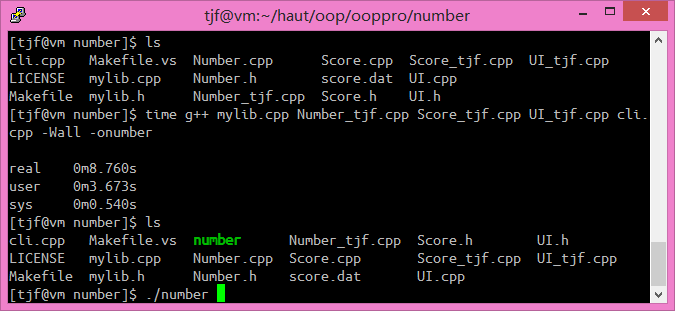
\includegraphics[width=\textwidth]{image/tjf/compile.png}
\caption{\label{compile}在 Linux 下的编译过程}
\end{figure}

如图~\ref{compile}~,使用 g++ 编译(当然也可以用 make 来调用)。可以看到 C++ 的编译是比较慢的,这里花了有 8 秒多才把这 500 多行程序编译完。平常编译安装软件的时候也比较害怕遇到 C++ 的,因为总是 make 之后就是一个下午的等待了。而 C 的编译比这要快得多。这也是 C++ 语言固有的缺陷。

%\begin{figure}[htp]
%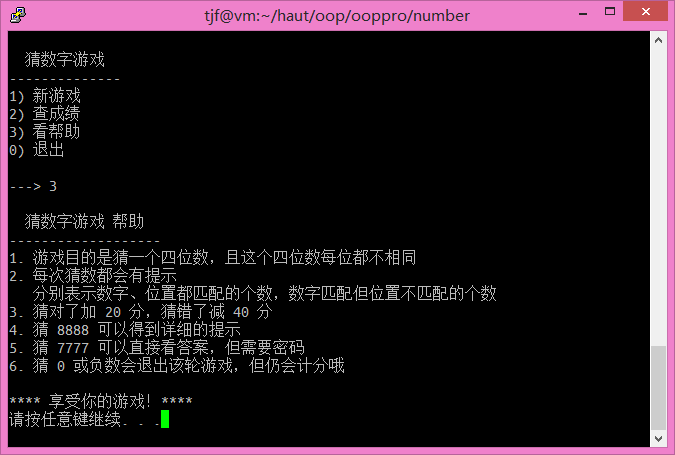
\includegraphics[width=\textwidth]{image/tjf/help.png}
%\caption{\label{help}帮助界面}
%\end{figure}

%运行程序,进入主界面后选择查看帮助,则会显示如图~\ref{help}~的帮助信息。

\begin{figure}[htp]
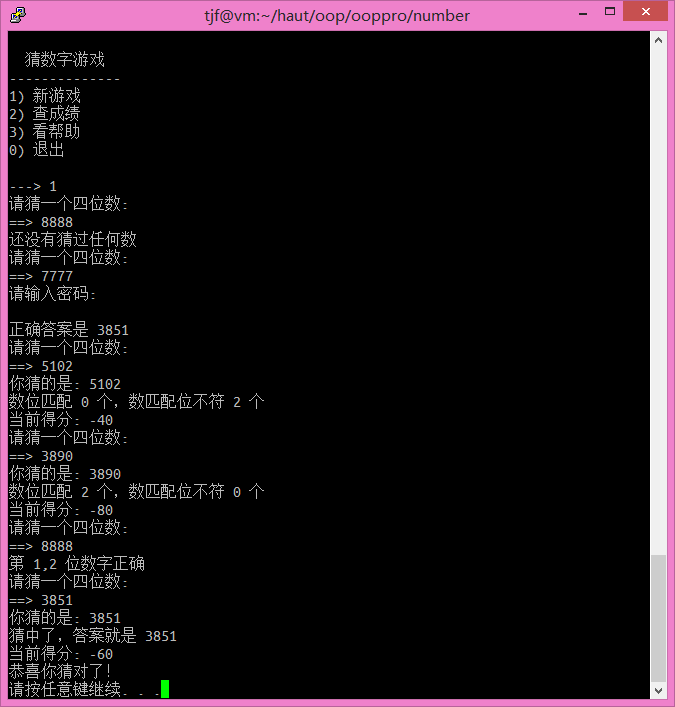
\includegraphics[width=\textwidth]{image/tjf/guess.png}
\caption{\label{guess}在 Linux 下执行一个猜数流程}
\end{figure}

如图~\ref{guess}~,我执行了一个猜数流程。可以看到程序根据不同的输入做出了合适的回应,当输入 7777 时要求输入密码并给出了答案;输入 8888 则会在有过往输入的情况下显示详细提示;对于正常的输入会显示正常的提示信息 $(x,y)$ 数对;猜对了后会暂停并等待按下任意键。

这里可以注意到输入密码时并没有回显,这和往常在 Windows 下输入后回显星号“*”不一样。在 Linux 的惯例是不回显密码的,为了适应这一不同,我在 mylib 中提供的函数也根据预编译参数编译了针对不同操作系统的代码。

\subsection{Windows 下的运行情况}

这个程序是由\xzp 编写,在 Windows 上使用 Visual Studio 2013 编译生成可执行文件,由\wzh 进行测试并截图的。

\begin{figure}[htp]
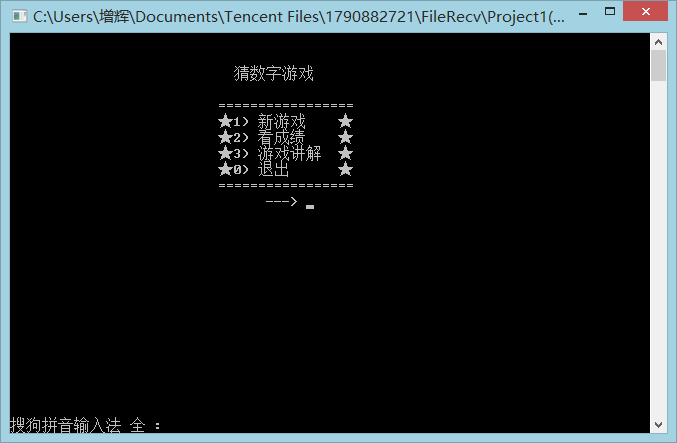
\includegraphics[width=\textwidth]{image/21.png}
\caption{\label{p1}运行程序后,出现此界面。输入1,进入游戏。输入2,查看游戏成绩。输入3,可查看详细的游戏讲解。输入0,则会退出游戏。}
\end{figure}

如图~\ref{p1}~,运行程序后,出现此界面。输入1,进入游戏。输入2,查看游戏成绩。输入3,可查看详细的游戏讲解。输入0,则会退出游戏。

\begin{figure}[htp]
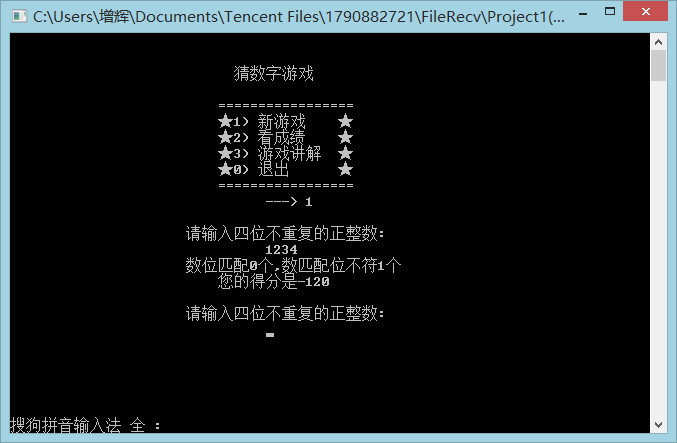
\includegraphics[width=\textwidth]{image/22.png}
\caption{\label{p2}按要求输入1后,开始游戏,输入四个不重复的正整数后,显示数位匹配及数位不匹配的个数,以及所得分数。如果猜数不正确,则继续游戏。}
\end{figure}

如图~\ref{p2}~,按要求输入1后,开始游戏,输入四个不重复的正整数后,显示数位匹配及数位不匹配的个数,以及所得分数。如果猜数不正确,则继续游戏。

\begin{figure}[htp]
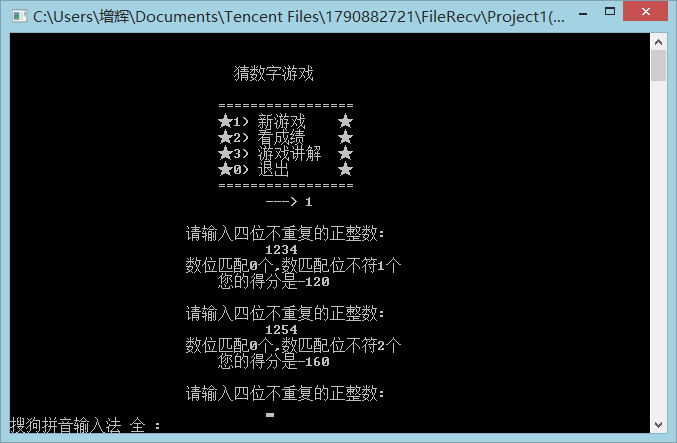
\includegraphics[width=\textwidth]{image/23.png}
\caption{\label{p3}再次输入,没有猜对数字,提示继续游戏。}
\end{figure}

如图~\ref{p3}~,再次输入,没有猜对数字,提示继续游戏。

\begin{figure}[htp]
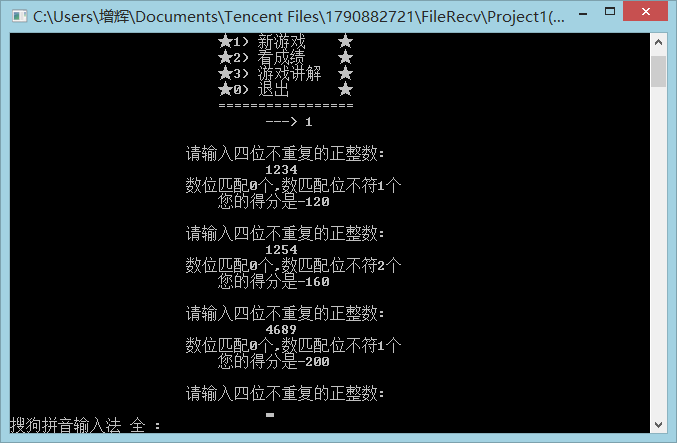
\includegraphics[width=\textwidth]{image/24.png}
\caption{\label{p4}输入数字,没有猜对数字,提示继续游戏。}
\end{figure}
 
如图~\ref{p4}~,输入数字,没有猜对数字,提示继续游戏。

\begin{figure}[htp]
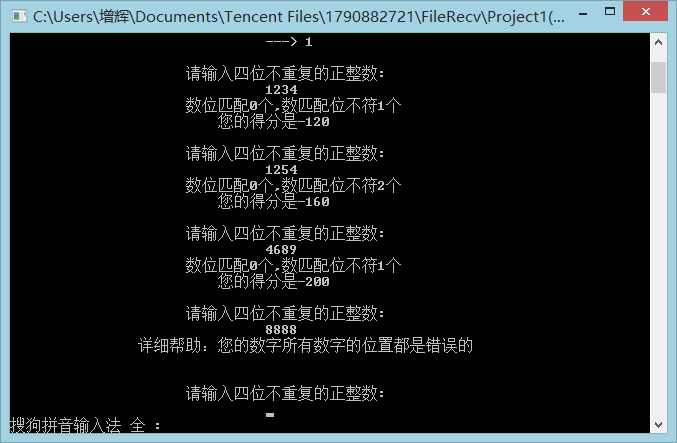
\includegraphics[width=\textwidth]{image/25.png}
\caption{\label{p5}输入8888,得到更详细的帮助信息。系统会提示第几位数字正确。}
\end{figure}
 
如图~\ref{p5}~,输入8888,得到更详细的帮助信息。系统会提示第几位数字正确。
 
\begin{figure}[htp]
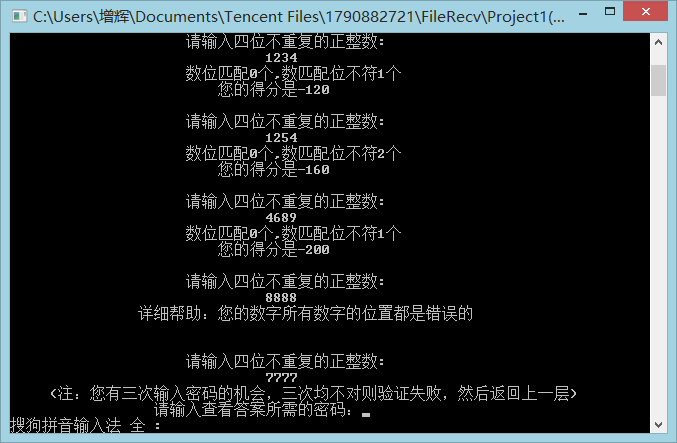
\includegraphics[width=\textwidth]{image/26.png}
\caption{\label{p6}获得系统所给出的正确数字,但要求输入密码,密码正确后方可得到正确数字,并且只有三次输入密码的机会。}
\end{figure}
 
如图~\ref{p6}~,输入7777,获得系统所给出的正确数字,但要求输入密码,密码正确后方可得到正确数字,并且只有三次输入密码的机会。

\begin{figure}[htp]
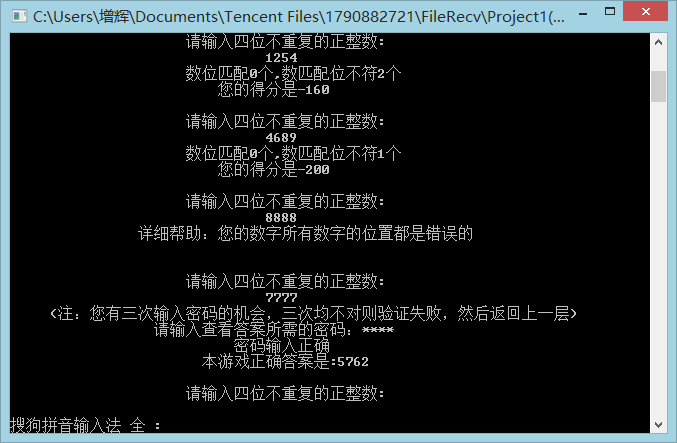
\includegraphics[width=\textwidth]{image/27.png}
\caption{\label{p7}输入正确的密码后,得到游戏的正确答案。}
\end{figure}
 
如图~\ref{p7}~,输入正确的密码后,得到游戏的正确答案。

\begin{figure}[htp]
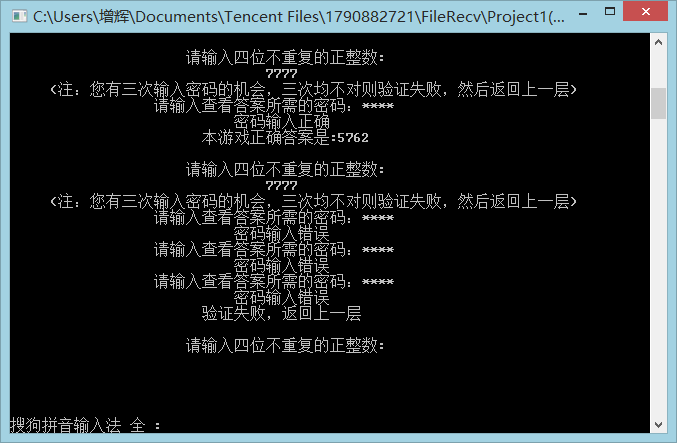
\includegraphics[width=\textwidth]{image/28.png}
\caption{\label{p8}三次密码输入错误后,提示验证失败,返回上一级,继续进行游戏。}
\end{figure}
 
如图~\ref{p8}~,三次密码输入错误后,提示验证失败,返回上一级,继续进行游戏。

\begin{figure}[htp]
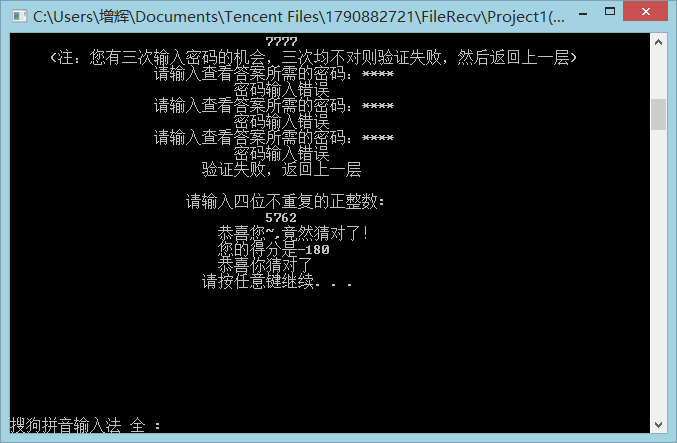
\includegraphics[width=\textwidth]{image/29.png}
\caption{\label{p9}输入正确的答案后,系统提示猜对。并给出所得分数。}
\end{figure}
 
如图~\ref{p9}~,输入正确的答案后,系统提示猜对。并给出所得分数。

\begin{figure}[htp]
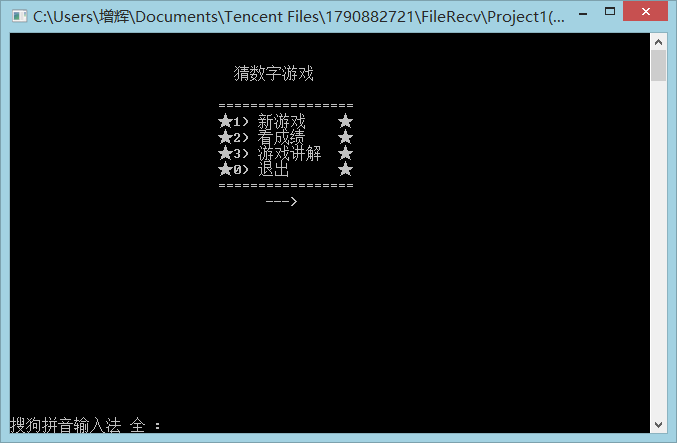
\includegraphics[width=\textwidth]{image/30.png}
\caption{\label{p10}猜对数字后,按任意键,出现此界面。输入1,进入游戏。输入2,查看游戏成绩。输入3,可查看详细的游戏讲解。输入0,则会退出游戏。}
\end{figure}
 
如图~\ref{p10}~,猜对数字后,按任意键,出现此界面。输入1,进入游戏。输入2,查看游戏成绩。输入3,可查看详细的游戏讲解。输入0,则会退出游戏。

\begin{figure}[htp]
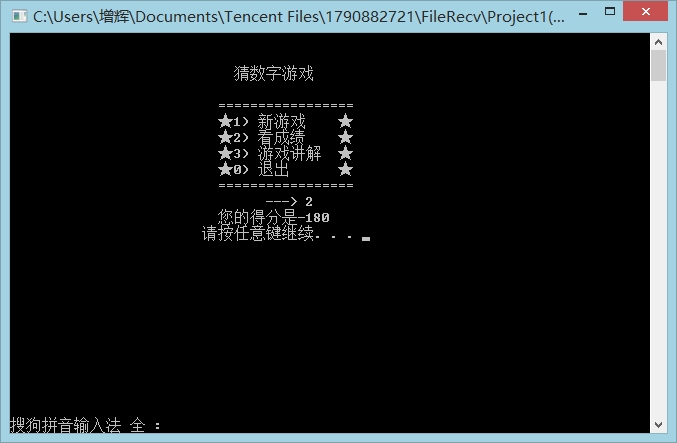
\includegraphics[width=\textwidth]{image/31.png}
\caption{\label{p11}猜对数字后,按任意键,出现开始界面。输入2,可查看上轮游戏成绩。}
\end{figure}
 
如图~\ref{p11}~,猜对数字后,按任意键,出现开始界面。输入2,可查看上轮游戏成绩。

\begin{figure}[htp]
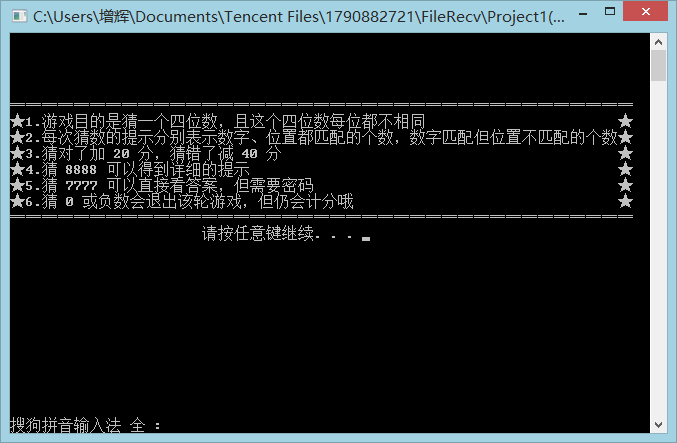
\includegraphics[width=\textwidth]{image/32.png}
\caption{\label{p12}输入3,得到详细的游戏讲解。}
\end{figure}
 
如图~\ref{p12}~,输入3,得到详细的游戏讲解。
